\section*{Exercises}

\begin{description}
 \item[2.1-1] Ilustrate the operation of Insertion-Sort on the array $A = \{31,41,59,26,41,58\}$
\end{description}
\begin{center}
 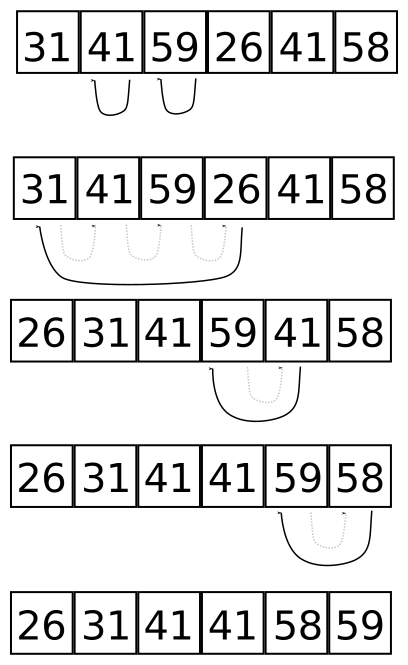
\includegraphics[width=100px]{chapter2/insertion_sort.pdf}
 % 2.1-1.png: 39x65 pixel, 9dpi, 11.02x18.36 cm, bb=0 0 312 520
\end{center}

\begin{description}
 \item[2.1-2] Rewrite the Insertion-Sort into nonincreasing instead of nondecreaseing order.
\end{description}

\lstset{language=python,
 backgroundcolor=\color{white},   % choose the background color; you must add \usepackage{color} or \usepackage{xcolor}
  basicstyle=\footnotesize,        % the size of the fonts that are used for the code
  breakatwhitespace=false,         % sets if automatic breaks should only happen at whitespace
  breaklines=true,                 % sets automatic line breaking
  captionpos=b,                    % sets the caption-position to bottom
  commentstyle=\color{mygreen},    % comment style
  deletekeywords={...},            % if you want to delete keywords from the given language
  escapeinside={\%*}{*)},          % if you want to add LaTeX within your code
  extendedchars=true,              % lets you use non-ASCII characters; for 8-bits encodings only, does not work with UTF-8
  frame=single,                    % adds a frame around the code
  keepspaces=true,                 % keeps spaces in text, useful for keeping indentation of code (possibly needs columns=flexible)
  keywordstyle=\color{blue},       % keyword style
  language=Octave,                 % the language of the code
  morekeywords={*,...},            % if you want to add more keywords to the set
  numbers=left,                    % where to put the line-numbers; possible values are (none, left, right)
  numbersep=5pt,                   % how far the line-numbers are from the code
  numberstyle=\tiny\color{mygray}, % the style that is used for the line-numbers
  rulecolor=\color{black},         % if not set, the frame-color may be changed on line-breaks within not-black text (e.g. comments (green here))
  showspaces=false,                % show spaces everywhere adding particular underscores; it overrides 'showstringspaces'
  showstringspaces=false,          % underline spaces within strings only
  showtabs=false,                  % show tabs within strings adding particular underscores
  stepnumber=2,                    % the step between two line-numbers. If it's 1, each line will be numbered
  stringstyle=\color{mymauve},     % string literal style
  tabsize=2,                       % sets default tabsize to 2 spaces
  title=\lstname                   % show the filename of files included with \lstinputlisting; also try caption instead of title
}
\begin{lstlisting}
def inverse_sort1(A):
    for j in range(1, len(A)):
        key = A[j] 
        i = j - 1  

        while i >= 0 and A[i] < key:
            A[i+1] = A[i]
            i = i - 1
        A[i+1] = key
    return A


def inverse_sort2(A):
    for j in range(1, len(A)):
        key = A[j] 
        i = j - 1 

        while i >= 0 and A[i] < A[i+1]:
            A[i+1] = A[i]
            A[i] = key
            i = i - 1
    return A
\end{lstlisting}


\begin{description}
 \item[2.1-3] Lineal searching problem.
\end{description}

\begin{lstlisting}
for i = 1 to A.length
    if A[i] = = v
	return i
return Nil
\end{lstlisting}

\begin{list}{}{}
 \item[Initialization:] Before the first iteration the subarray $A$ is empty so it could return $Nil$.
 \item[Maintenance:] Before an iteration the value $A[i]$ could be $v$ or not, to the output can be either the index $i$ or $Nil$.
 \item[Termination:] It the last item is not equal to $v$ then the algorithm should return $Nil$.
\end{list}

\begin{description}
 \item[2.1-4] Lineal searching problem.
\end{description}
\begin{lstlisting}
for i = 1 to n
    sum = A[i] + B[i]
    C[i] = sum
return C
\end{lstlisting}
\begin{list}{}{}
 \item[Initialization:] Before the first iteration no numbers were added so the array $C$ is returned as empty.
 \item[Maintenance:] Before an iteration the items in array $C$ should contain those that were added from the same index in the $A$ and $B$ arrays.
 \item[Termination:] After all items were added and included, the array $C$ will be returned.
\end{list}